\section{Design}
\label{section:design}

In this section we describe the design of our classes and algorithms based on
the requirements established in Section \ref{section:requirements}.

\subsection{Subsetter User Interface}

The subsetter is the first in a series of planned parallel command-line tools
based on unstructured grids, the PGAS model, and one-sided communication.  It
takes arguments indicating specific variables (-v), dimension ranges (-d) to
extract, or a latitude and longitude bounding box (-b).  Parallel climate
analysis tools require the use of common startup programs (such as "mpirun" or
"mpiexec" for MPI programs) capable of spawning parallel jobs on a cluster of
other parallel architecture.  Users of these tools must become familiar with
how to run parallel software.  Looking past the particular use of "mpiexec
-np" below to invoke our MPI program with a given number of processors,
example usage of the subsetter looks like:

\begin{itemize}
\item mpiexec -np 128 subsetter -b 20,-20,160,90 -v vorticity january.nc february.nc MJO\_vorticity\_janfeb.nc
\item mpiexec -np 64 subsetter -b 90,0,180,-180 -d levels,1,5 geopotential.nc out.nc
\end{itemize}

Similarly, the NetCDF Operator's \emph{ncks} application\cite{NCO} is run
like the following, noting that \emph{ncks} does not aggregate input files:

\begin{itemize}
\item ncks -X 90,160,-20,20 -v vorticity january.nc MJO\_vorticity\_january.nc
\item ncks -X -180,180,0,90 -d levels,1,5 geopotential.nc out.nc
\end{itemize}

\subsection{Dataset Abstraction}

A dataset abstraction is essential for the comprehension of these large
datasets, hiding the details of which files contain which data.  The subsetter
currently supports two forms of input file aggregation, either across a
specified dimension e.g. time or by taking the union of all input files such
that duplicate dimensions and grid and topology variables within later files
are ignored.  These forms of aggregation are modeled after what is available
when using NetCDF Markup Language\cite{NcML}.  NcML input is not directly
supported at this time but is planned for a future release. 

\subsection{Parallel IO Abstraction}

IO operations are hidden behind abstract base classes.  Any IO library can be
supported so long as the data structures conform to the Common Data Model
(CDM)\cite{CDM}.  This is similar to how the Java NetCDF library works,
supporting many different data formats conforming to the CDM\cite{JavaNetCDF}.
Further, differing IO strategies using the same IO library can also be
developed behind the same API.  The use of Parallel-NetCDF was selected
because of the ubiquity of the NetCDF libraries and data format in climate
applications.

\subsection{The Global Arrays Library}

The PGAS programming model assumes a global address space which is partitioned
such that each process is associated with a local portion of the space.
One-sided communication allows a process to access another process's address
space without any explicit participation by the latter process.  Such
communication can reduce synchronization and can simplify programming.  The
Global Arrays (GA) library supports both global address spaces and onesided
communication.

The subsetter was built using the GA library for the wealth of features it
provides which are tailored to our problem domain.  GA provides a distributed
dense multidimensional array programming abstraction and the data we will be
operating over is stored as dense arrays within NetCDF files.  It should be
noted that dense distributed arrays would also work well for regularly gridded
data.  However, due to the use of unstructured grid data, the algorithm for
subsetting the data will look quite different than for the structured case.
Recall that for unstructured grids, logically adjacent cells are not
necessarily adjacent in memory.  In order to evenly distribute a subset, a
single process will need to send a varying amount of data to any number of
other processes.  Certainly a collective operation could be considered, but GA
provides the necessary functionality without needing any explicit cooperation
from any other process.  Any given process will simply put the section of the
subset into the remote process's memory which owns the subset.

There are certain GA one-sided operations which are tailored for use on
one-dimensional arrays which are used within our program.  These operations
include:

\begin{itemize}
\item \verb=GA_Patch_enum=,
\item \verb=GA_Scan_add=, and
\item \verb=GA_Unpack=
\end{itemize}

Those operations have been demonstrated in the computation of sparse matrix
multiplication\cite{GA} but are equally useful in the manipulation of
unstructured grids.  The remaining GA operations are N-dimensional and
include:

\begin{itemize}
\item \verb=NGA_Scatter=,
\item \verb=NGA_Gather=,
\item \verb=NGA_Put=, and
\item \verb=NGA_Get=
\end{itemize}

Those operations are useful for redistributing the subset data and for
querying the values of the various distributed arrays without regard to which
process owns the data being queried.

\subsection{The Algorithms}

The one-sided communication and PGAS model supported by GA allowed us to
develop some novel algorithms for the manipulation of unstructured grids.  In
this section we diagram and describe the algorithms we developed.  The vast
majority of functionality within the subsetter is provided by either
Parallel-NetCDF or GA.  GA allocates and evenly distributes the arrays.  The
starting and ending indices owned by each process are used directly to fill
the arrays using Parallel-NetCDF.  GA operations are then used to prepare the
data for packing, at which point a custom n-dimensional packing routine is
used.  After packing, evenly-distributed data is written back to disk using
Parallel-NetCDF.  (Note that instead of immediately writing the data back to
disk, any number of other mathematical operations could take place.) Of these
algorithms, the novel ones include reindexing the masks, reindexing the
topology variables, and the n-dimensional pack routine.

Each dimension of the data has two arrays associated with it, an integer array
representing a bitmask and an integer array representing the new indices of
<<<<<<< .mine
the dimension in case of a subset.  For instance, if any of the bits are
zero (off), the corresponding indices of the index array will have negative
values.  The remaining values of the index array will increase monotonically,
skipping the negative or masked indices.  The bitmasks are generated based on
a rectangular latitude and longitude region specified on the command-line, or
by specifying one or more indices of a dimension to select. Although the
bitmasks are currently created using a relatively simple latitude-longitude
bounding box, arbitrary bitmasks could be created and fed into the subsetter
without modification of the remaining algorithms. This would allow for data sets
based on feature extraction (e.g. cyclones) or continental datasets.
These bitmasks are then
=======
the dimension in case of a subset.  For instance, if any of the bits are zero
(off), the corresponding indices of the index array will have negative values.
The remaining values of the index array will increase monotonically, skipping
the negative or masked indices.  The bitmasks are generated based on a
rectangular latitude and longitude region specified on the command-line, or by
specifying one or more indices of a dimension to select.  Although a
rectangular region is currently used for simplicity, once translated the
bitmasks allow for arbitrary subsets to be defined.  These bitmasks are then
>>>>>>> .r218
used to evenly distribute the resultant subset across all processes.  Note
that these bitmask and associated index arrays are one-dimensional and
distributed.

\subsubsection{Partial Sum}

%\begin{figure}[!t]
%\center
%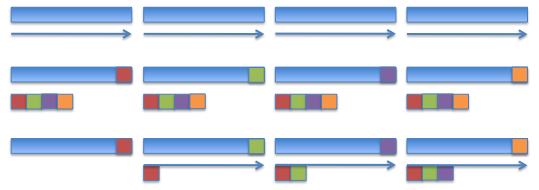
\includegraphics[width=3.5in]{images/partialsum}
%\caption{A distributed partial sum over a 1-D array.  A partial sum is first
%computed over the local portions (A), the last values of each portion are
%collected on each process (B), and lastly each local portion adds the last
%values taken from each previous process (C).}
%\label{fig:partialsum}
%\end{figure}

A partial sum of the index array associated with each dimension is useful for
<<<<<<< .mine
later determining where subset data is to be placed.  That feature will be
explained in more detail in Section \ref{section:alg_pack}.  The partial sum
operation here is semantically similar to the one found in the C++
STL\cite{CXXSTL}.  It computes a series of sums over an array from the first
element through the \emph{i}th element and stores the result of each such sum
in the \emph{i}th element of a destination array.  For example, if $x$
represents an element in the source array and $y$ represents an element in the
destination array, the $y$s can be calculated as:
=======
later determining which process is to receive which portion of the subset
data.  That feature will be explained in more detail in Section
\ref{section:alg_pack}.  The partial sum operation here is semantically
similar to the one found in the C++ STL\cite{CXXSTL}.  It computes a series of
sums over an array from the first element through the \emph{i}th element and
stores the result of each such sum in the \emph{i}th element of a destination
array.  For example, if $x$ represents an element in the array and $y$
represents an element in the destination array, the $y$s can be calculated as:
>>>>>>> .r218

\begin{equation}
\begin{split}
y_0 &= x_0\\
y_1 &= x_0 + x_1\\
y_2 &= x_0 + x_1 + x_2\\
y_3 &= x_0 + x_1 + x_2 + x_3\\
\ldots
\end{split}
\end{equation}

%The partial sum is computed by first performing partial sums of each local
%portion of the source array.  This operation is represented by Fig.
%\ref{fig:partialsum}A.  The last value of each local sum is then collectively
%distributed to each process as seen in Fig. \ref{fig:partialsum}B.  Fig.
%\ref{fig:partialsum}C is the last step where each local portion adds the last
%values of each process's sum which come before.

The partial sum is elegantly computed using a single call to the
\verb+GA_Scan_add+ routine.

\subsubsection{Reindexing of Dimension Index}

Creating the index array associated with a mask requires three specific GA
operations, \verb=GA_Fill=, \verb=GA_Patch_enum= and \verb=GA_Unpack=.  The
mask array is represented in Fig. \ref{fig:unpack}A with the masked bits
indicated in black.  \verb=GA_Fill= fills the index array, the array in Fig.
\ref{fig:unpack}B, with a value of $-1$.  Each process counts how many masked
bits they own and then collectively sums their count.  A third array is
created (Fig. \ref{fig:unpack}C) based on this count.  \verb=GA_Patch_enum=
enumerates the values in the newly created array starting from zero with an
increment of 1 (indicated by the arrows in Fig. \ref{fig:unpack}C).
\verb=GA_Unpack= expands the enumerated array values into the filled array
based on the associated mask array as seen in Fig. \ref{fig:unpack}D.

\begin{figure}[!t]
\center
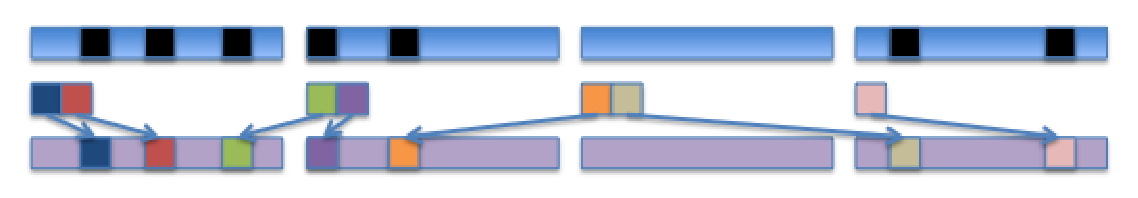
\includegraphics[width=3.5in]{images/unpack}
\caption{Reindexing of a Dimension Index.  The index array (B) is filled with
a value of $-1$.  The masked bits of (A) are tallied such that a new array (C)
is created based on the tallied size.  The new array C is enumerated and then
unpacked into the index array (D).}
\label{fig:unpack}
\end{figure}

\subsubsection{Reindexing of Topology Variables}

Recall that the topology variables are those which map from one index to one
or more other indices such as from a cell index to each of its corner indices.
A typical subset operation reduces the number of cells, corners, and edges
within the grid, so it is important to maintain the integrity of these mapping
arrays such that they map to real indices.

The reindexing of the topology variables relies on the recalculated index
array of the associated domain.  For example, when reindexing the mapping from
edges to corners, the recalculated corners index array is required (Fig.
\ref{fig:reindex}A).  The mapping values represent indices into the
recalculated index array.  The original mapping arrays are iterated over to
prepare the required indices for the subsequent GA routine \verb=NGA_Gather=
to query.  The \verb=NGA_Gather= routine gathers array elements from a global
array into a local array by specifying the desired indices.  In this way each
process gathers the new values for the mapping from the index array and then
appropriately replaces the old mapping values.  For clarity, Fig.
\ref{fig:reindex}B shows four processes gathering and replacing only the
non-negative indices, but it should be noted that all indices are replaced by
this operation.

\begin{figure}[!t]
\center
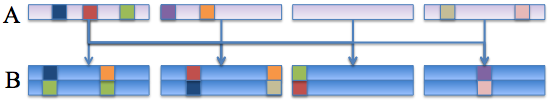
\includegraphics[width=3.5in]{images/reindex2}
\caption{Reindexing of Topology Variables.  The recalculated index array from
the Fig. \ref{fig:unpack} reindexing operation, seen here as (A), will replace
values found within the topology array (B).  Each process gathers values from
the index array after using the original values from (B) in an NGA\_Gather
call.  All values from the original index array are replaced (only replacement
of non-negative indices is shown for clarity).}
\label{fig:reindex}
\end{figure}

\subsubsection{N-Dimensional Pack}
\label{section:alg_pack}

The goal of the pack routine is to start with an evenly distributed source
array, subset it, and evenly distribute the subset.  The subset is specified
using mask arrays, one for each dimension of the source array (the blue arrays
in Fig. \ref{fig:pack} with masked bits indicated in black).  The size of the
subset is determined by counting the number of masked bits per dimension.
Each process determines where to \verb=NGA_Put()= its portion of the subset by
examining the partial sum array (the olive arrays in Fig. \ref{fig:pack}).
The values indicated in orange in Fig. \ref{fig:pack} represent the values of
partial sum array at those particular indices and are used by each process to
know where to put their portion of the subset data into the subset array.  For
example, process 1 in Fig. \ref{fig:pack} calls \verb=NGA_Put()= to place its
data starting at index (3,0).

The partial sum of the mask array is a convenient solution to this problem.
Each process owns a portion of the source array in terms of the global address
space of the array.  For each dimension, the value in the corresponding
partial sum array at the index represented by the lowest index owned by each
local portion describes where to put the subset data.

Fig. \ref{fig:pack} illustrates the n-dimensional pack routine schematically.
In the figure, the blue arrays represent the mask arrays and the olive arrays
the partial sums.  The masked bits are indicated in black.  Each of the four
processes query the partial sum arrays using \verb=NGA_Get()= at the
corresponding locations indicated in orange and the small blue arrows.  Now
knowing where to put their subset data, each process can pack their data into a
small local block and then \verb=NGA_Put()=
the resulting portions into the final subset array.  The \verb=NGA_Get()= and
\verb=NGA_Put()= operations do not require explicit knowledge of where the
data lives, reducing the burden of the programmer.

\begin{figure}[!t]
\center
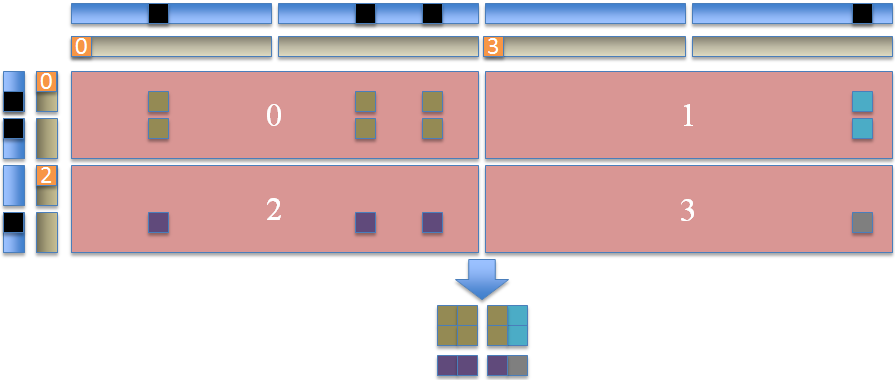
\includegraphics[width=3.5in]{images/pack}
\caption{Pack.  The blue arrays represent the masks with masked bits indicated
in black.  The olive arrays are the partial sums over the masks.  The orange
values represent the values of the partial sum array at those indices.  Each
process queries the partial sum arrays for where to put their subset data,
packs their local data based on the mask bits, and calls NGA\_Put to deliver
the subset data.  The destination array is by default evenly distributed.}
\label{fig:pack}
\end{figure}

The data location abstraction offered by GA is even more important as
differing numbers of processors and/or different data distributions are used.
As can be seen in the case diagrammed in Fig. \ref{fig:pack}, the partial sum
arrays are as evenly distributed as the data arrays.  Although GA evenly
distributes arrays by default, different distributions can be specified.  For
example, it might be beneficial to keep all vertical levels for a given region
local to a process.  The desired values from the partial sum arrays will
change process owners depending on how many processes are used or how the data
is distributed.  \verb+GA_Get+ and \verb+GA_Put+ abstract away that need to
track which process owns the data and simplifies the programming model.
